\documentclass[10pt]{article}

\pagestyle{empty}

\setlength{\textheight}{250mm}
\setlength{\textwidth}{180mm}
\setlength{\oddsidemargin}{-8mm}
\setlength{\topmargin}{-1.5cm}

\usepackage{amsmath}
\usepackage{amsthm}
\usepackage{psfrag}
\usepackage{graphicx}
\usepackage{bm}
\usepackage{mathrsfs}
\usepackage{icomma} % pacchetto per limitare lo spazio standard posto dopo la virgola in caso che la virgola sia tra cifre
\usepackage{amsfonts} % amplia i caratteri matematici disponibili
\usepackage{amssymb}
%\usepackage{wrapfig}
\usepackage{empheq}

\usepackage{epstopdf}
\usepackage[utf8x]{inputenc}
\usepackage{ifthen}

\usepackage{caption}

\usepackage[italian]{babel}
%\usepackage[latin1]{inputenc}

\usepackage{subfig}

\usepackage{pgfplots}
\pgfplotsset{compat=1.9}

%\input{def}

%\newcommand{\kg}{\textrm{kg}}
%\newcommand{\K}{\textrm{K}}
%\newcommand{\m} {\textrm{m}}
%\newcommand{\dm}{\textrm{dm}}
%\newcommand{\cm}{\textrm{cm}}
%\newcommand{\mm}{\textrm{mm}}
%\newcommand{\s} {\textrm{s}}
%\newcommand{\N} {\textrm{N}}
%\renewcommand{\Pa}{\textrm{Pa}}

\def \flagSect{0} % 1    : numerazione
		  % else : niente
%\newcommand{\taitol}[1]  % stile titolo
%{
%%{\textit{#1}}
%{#1}
%}
\def \soluzione{Soluzione}
\def \partePrima{Concetti. }
\def \parteSeconda{Svolgimento. }
%\def \parteTerza{}
\newcommand{\sol}{\subsubsection*{\soluzione}}
\newcommand{\partone}{\ \ \ \ \ \textbf{\partePrima}}
\newcommand{\parttwo}{\vspace{0.2cm}\textbf{\parteSeconda}}

\ifnum\flagSect=1
\newtheorem{esercizio}{Esercizio}%[section]
\else
\newtheorem*{esercizio}{Esercizio}
\fi

\newtheorem*{teorema}{Teorema}
\newtheorem*{lemma}{Lemma}

% ###########################################################
%\def \flagSect{0} % 1    : numerazione
		  % else : niente
%\newcommand{\taitol}[1]  % stile titolo
%{
%%{\textit{#1}}
%{#1}
%}
\def \soluzione{Soluzione}
\def \partePrima{Concetti. }
\def \parteSeconda{Svolgimento. }
%\def \parteTerza{}
\newcommand{\sol}{\subsubsection*{\soluzione}}
\newcommand{\partone}{\ \ \ \ \ \textbf{\partePrima}}
\newcommand{\parttwo}{\vspace{0.2cm}\textbf{\parteSeconda}}

\ifnum\flagSect=1
\newtheorem{esercizio}{Esercizio}%[section]
\else
\newtheorem*{esercizio}{Esercizio}
\fi

\newtheorem*{teorema}{Teorema}
\newtheorem*{lemma}{Lemma}

% ###########################################################
%\def \flagSect{0} % 1    : numerazione
		  % else : niente
%\newcommand{\taitol}[1]  % stile titolo
%{
%%{\textit{#1}}
%{#1}
%}
\def \soluzione{Soluzione}
\def \partePrima{Concetti. }
\def \parteSeconda{Svolgimento. }
%\def \parteTerza{}
\newcommand{\sol}{\subsubsection*{\soluzione}}
\newcommand{\partone}{\ \ \ \ \ \textbf{\partePrima}}
\newcommand{\parttwo}{\vspace{0.2cm}\textbf{\parteSeconda}}

\ifnum\flagSect=1
\newtheorem{esercizio}{Esercizio}%[section]
\else
\newtheorem*{esercizio}{Esercizio}
\fi

\newtheorem*{teorema}{Teorema}
\newtheorem*{lemma}{Lemma}

% ###########################################################
%\input{logicNumb}
%\newcommand{\sectionIf}[2]
%{
%   \ifthenelse{\equal{#1}{1}}
%              {\subsection{#2}}{\subsection*{#2}}
%}
% ###########################################################

%\newcommand{\sectionIf}[2]
%{
%   \ifthenelse{\equal{#1}{1}}
%              {\subsection{#2}}{\subsection*{#2}}
%}
% ###########################################################

%\newcommand{\sectionIf}[2]
%{
%   \ifthenelse{\equal{#1}{1}}
%              {\subsection{#2}}{\subsection*{#2}}
%}
% ###########################################################


\begin{document}

\begin{center}
\textbf{Esercizi per il corso di Fluidodinamica} 
\medskip
\end{center}


\noindent
\begin{tabular}{cc}
\begin{minipage}{0.60\textwidth}
\begin{exerciseS}[Lamina in moto uniforme in canale piano]
Una lastra piana di lunghezza e apertura infinita si spessore 
$t=1\ mm$ scorre in un canale piano di altezza $H=2.22\  mm$
contenente acqua in condizioni standard. 
Essa viene mantenuta a distanza costante $h_1=0.5\  mm$ dalla parete
superiore e si muove a velocit\`a constante $U=0.55 \  m/s$.

Calcolare:
\begin{itemize}
\item il numero di Reynolds basato sulla velocit\`a $U$ della parete
e sulla distanza fra le pareti sia per la porzione di corrente superiore
sia per quella inferiore;
\item la componente orizzontale del risultante delle forze per unit\`a di
superficie esercitate dal fluido sulla lamina;
\item la potenza per unit\`a di superficie che occorre fornire alla 
lastra per mantenerla in moto uniforme.
\end{itemize}


($ Re_{sup}=239$, 
 $ Re_{inf}=344$, 
 $F_x=-2.14\ N/m^2$, 
 $P=1.17\  W/m^2$)
\end{exerciseS}
\end{minipage}
&
\begin{minipage}{0.35\textwidth}
   \begin{center}
   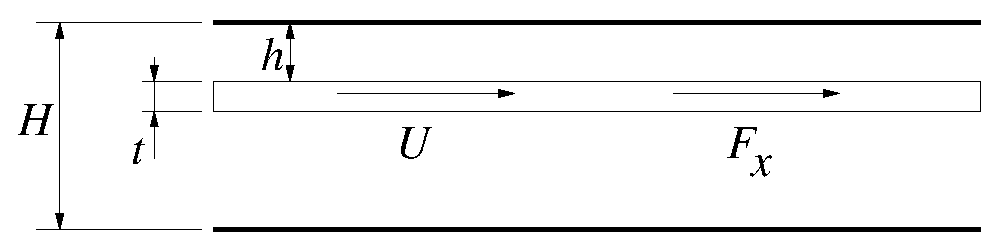
\includegraphics[width=0.70\textwidth]{./fig/lastracanale.eps}
   \end{center}
\end{minipage}
\end{tabular}

\sol

\partone Soluzioni esatte delle equazioni di Navier-Stokes. Corrente di Newton.

\parttwo La soluzione del problema può essere ricondotta alla soluzione esatta
della corrente di Newton nel canale piano. Si può calcolare immediatamente il numero
di Reynolds basato sulle due diverse lunghezze di riferimento, poichè densità e viscosità
sono date e la velocità di riferimento del problema è quella della lastra, nota anch'essa.

In seguito, si calcola lo sforzo a parete per ricavare la forza per unità di superficie esercitata
dal fluido sulla lamina e la potenza (prodotto di forza e velocità) necessaria a mantenere la 
lamina in moto uniforme.

\begin{itemize}

\item Numero di Reynolds
 \begin{equation}
   Re = \frac{\rho U L}{\mu}  \qquad \Rightarrow \qquad Re_{sup} = 239 , \quad Re_{inf} = 344
 \end{equation}

\item Scrivendo le equazioni per uno solo dei due lati, indicando con $z=0$ la coordinata della parete fissa
e $z=l$ quella della parete mobile, si ricava la corrente di Newton:
\begin{equation}
  u(z) = U \frac{z}{l}
\end{equation}

\item Il profilo di velocità per la corrente di Newton è lineare. Lo sforzo viscoso a parete (su una sola delle superfici)
vale 
\begin{equation}
  \tau_w = \mu \frac{U}{l}
\end{equation}

Sommando gli effetti su entrambe le pareti, la forza per unità di superficie si scrive come
\begin{equation}
  \frac{F}{S} = \tau = \mu U \displaystyle\left( \frac{1}{H-h-t} + \frac{1}{h} \right)
   \qquad \Rightarrow \qquad \tau = 2.14 N/m^2
\end{equation}

\item La potenza per unità di superficie si ricava dal prodotto della forza per unità di superfici
 e della velocità della lastra
\begin{equation}
  \frac{P}{S} = \frac{F}{S} U \qquad \Rightarrow \qquad \frac{P}{S} = 1.17 W/m^2
\end{equation}


\end{itemize}



%%%%%%%%%%%%%%%%%%%%%%%%%%%%%%%%%%%%%%%%%%%%%%%%%%%%%%%%%%%%%%%%%%

%%%%%%%%%%%%%%%%%%%%%%%%%%%%%%%%%%%%%%%%%%%%%%%%%%%%%%%%%%%%%%%%%%

%%%%%%%%%%%%%%%%%%%%%%%%%%%%%%%%%%%%%%%%%%%%%%%%%%%%%%%%%%%%%%%%%%


%%%%%%%%%%%%%%%%%%%%%%%%%%%%%%%%%%%%%%%%%%%%%%%%%%%%%%%%%%%%%%%%%%

%%%%%%%%%%%%%%%%%%%%%%%%%%%%%%%%%%%%%%%%%%%%%%%%%%%%%%%%%%%%%%%%%%
%%%%%%%%%%%%%%%%%%%%%%%%%%%%%%%%%%%%%%%%%%%%%%%%%%%%%%%%%%%%%%%%%%

\end{document}
